\documentclass[a4paper]{article}

\newcommand\tab[1][1cm]{\hspace*{#1}}
\newcommand{\norm}[1]{\left\lVert#1\right\rVert}
%% Language and font encodings
\usepackage[english]{babel}
\usepackage[utf8x]{inputenc}
\usepackage[T1]{fontenc}
\usepackage{enumitem}
\usepackage{amsfonts}
\usepackage{amssymb}
\usepackage{multirow}
\usepackage{comment}
\usepackage{enumitem}
\usepackage{amsmath}
\usepackage{parskip}
\usepackage{enumerate}

%% Sets page size and margins
\usepackage[a4paper,top=2cm,bottom=2cm,left=3cm,right=3cm,marginparwidth=1.75cm]{geometry}

%% Useful packages
\usepackage{amsmath}
\usepackage{graphicx}

\usepackage[colorlinks=true, allcolors=blue]{hyperref}

\title{\textbf{Cloud Development API Documentation}}
\author{Garrett Haley(haleyg), Alea Weeks(weeksr), \\[2mm] Daniel Domme(dommed), Ethan Patterson(patteret)}
\begin{document}
\maketitle
\pagebreak
\tableofcontents
\pagebreak
\section{API Architecture Design}
\begin{figure}[h!]
    \centering
    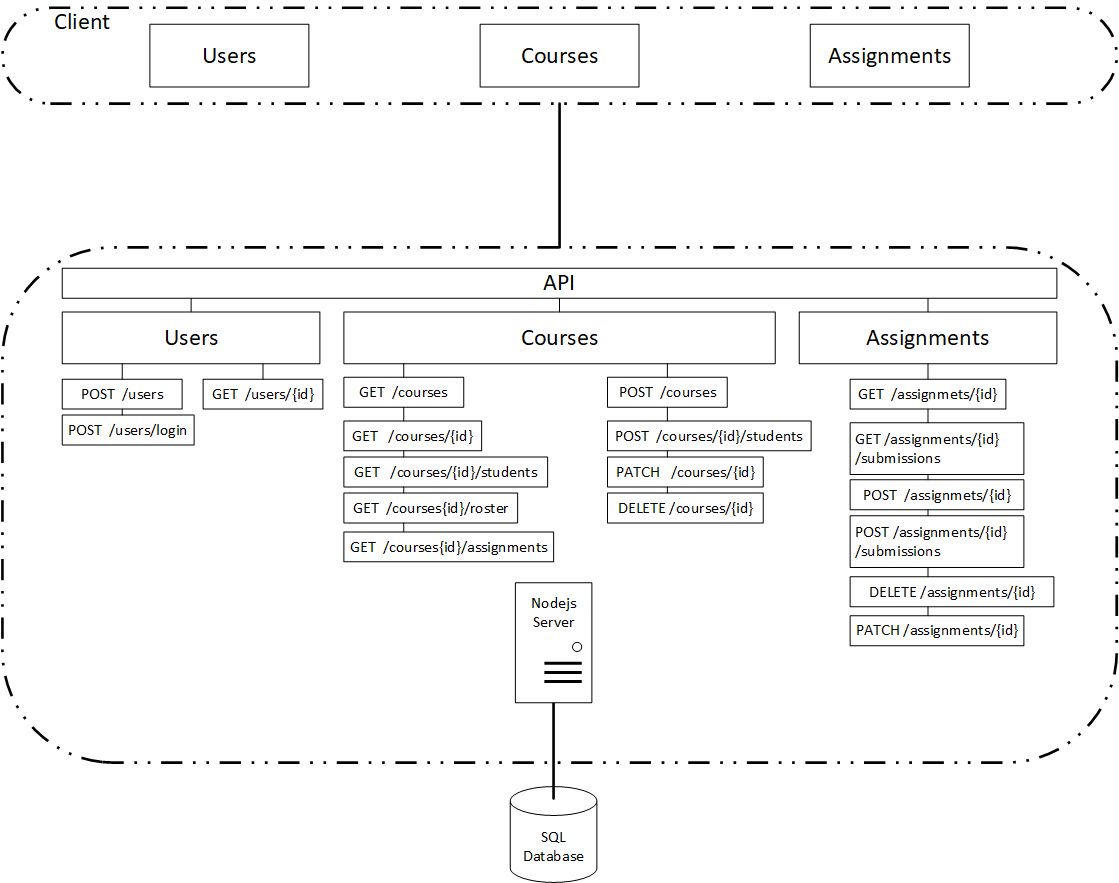
\includegraphics[scale=.4]{cloudAPI.png}
    \caption{API Design}
    \label{fig:my_label}
\end{figure}
The above diagram is a pictorial example of the current design of our system. The client has access to three endpoint objects for requesting information. These endpoint are users, courses, and assignments. All endpoints are accessed through a single nodejs. All data is stored securely in an SQL server that only the nodejs has privileges to access.
\\[2mm]
\parbox[t]{6.0in}{\raggedright%
\begin{enumerate}
  \item\textbf{Users endpoint}
  \begin{itemize}
    \item POST /users \# Adds a new user.\\[1mm]
    \item POST / users/login \# Allows a user to login.\\[1mm]
    \item GET /users/\{id\} \# Gets information for a specific user if authorized.\\[1mm]
  \end{itemize}
  \\[2mm]
  \item\textbf{Courses endpoint}
  \begin{itemize}
      \item GET /courses \# Fetches a list of courses.\\[1mm]
      \item GET /courses\{id\} \# Fetch data for a specific course.\\[1mm]
      \item GET /courses/\{id\}/students \# Fetch data for a specific course.\\[1mm]
      \item GET /courses\{id\}/roster \# Fetch a text/cvs file listing students in a course.\\[1mm]
      \item GET /courses/assignments \# Fetches a list of assignments for a course.\\[1mm]
      \item POST /courses \# Create a new course.\\[1mm]
      \item POST /courses/\{id\}/students \# Update enrolment for a specific course.\\[1mm]
      \item PATCH /courses/\{id\} \# Update data for a specific course.\\[1mm]
      \item DELETE /courses/\{id\} \# Remove a specific course.\\[1mm]
  \end{itemize}
  \\[2mm]
  \item\textbf{Assignments endpoint}
  \begin{itemize}
      \item POST /assignments \# Creates a new assignment.\\[1mm]
      \item POST /assignments/\{id\}submissions \# Creates a new submission for an assignment.\\[1mm]
      \item GET /assignments\{id\} \# Get information about a specific assignment.\\[1mm]
      \item GET /assignments/\{id\}submissions \# Fetch information about a specific assignment.\\[1mm]
      \item PATCH /assignments/\{id\} \# Update data for a specific assignment.\\[1mm]
      \item DELETE /assignments/\{id\} \# Remove a specific assignment.
  \end{itemize}
\end{enumerate}}
\newpage
\section{Data Schema}
\begin{figure}[h!]
    \centering
    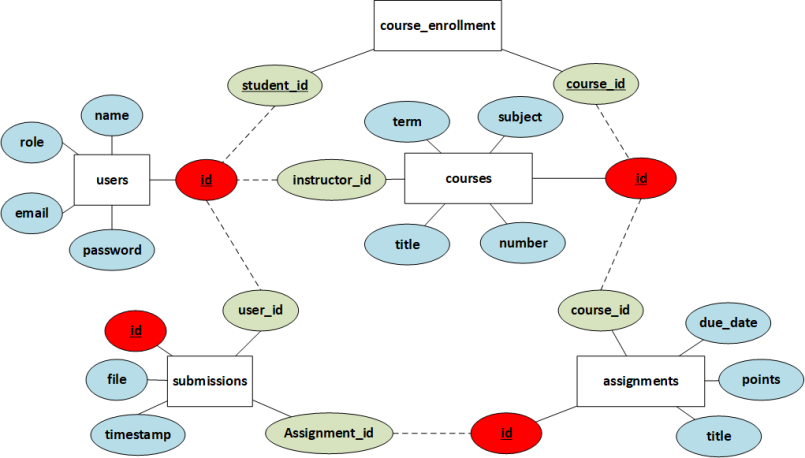
\includegraphics[scale=.4]{cloudER.png}
    \caption{Data Schema}
    \label{fig:my_label}
\end{figure}
Figure 2 depicts the data schema currently in use by our SQL database.
\begin{enumerate}
    \item White squares represent tables.\tab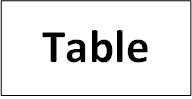
\includegraphics[scale=.2]{table.png}
    \item Red elements represent a unique id for a table.\tab
\includegraphics[scale=.2]{id.png}
    \item Blue elements represent attributes of a table.\tab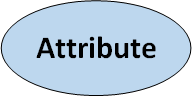
\includegraphics[scale=.2]{elem.png}
    \item Green elements represent foreign keys. All foreign keys have a dashed line connecting them to the location of their primary key.\tab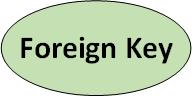
\includegraphics[scale=.2]{fk.png}
    \item Elements with underscores also represent primary keys. This allows foreign keys to be\newline primary.
\end{enumerate}
\section{Reflection}
\subsection{Design}
We chose the API architecture shown in figure 1 as we thought this would be the fastest and most efficient way of getting data to and from our database to the user. Because Tarpaulin needs to provide features similar to Canvas, we wanted to make sure that all updates requested to the Tarpaulin service are immediately updated for all others clients. For this reason the speed at which information is propagated in our system is critical. 
\par
\noindent
To achieve this goal our API server is implemented using nodejs. This allows our server to service multiple clients at a much faster rate than if it was implemented with a service designed using PHP. For information storage and retrieval we chose to implement our database using mysql. All resources suggested if speed is a concern, a SQL database would be the preferred option.
\par
\noindent
All request for information are first handled and processed by the single nodejs server. This server is then responsible for reaching out to the database to query for the requested information if the user meets all policies in place to access said information. Currently we have a rate limiter set for for 5 attempts over a 6 second time period. 

\par
\noindent
Currently admins have access to all information. Instructors can request less information than admins, but have far more access than a student. Instructors can currently post new assignments, get a list of student ids in a given class, add or remove students from a course, update a specific course, and request a course roster. The student role is the most restricted of the three. Users with the student role can submit assignments, and update assignments.
\newpage
\subsection{Things we would like to change}
We followed the instructions listed in the provided openapi file for every endpoint specification. Because we followed the specifications in this file so closely this made our database less than normalized, as you can see in the data schema in figure 2. We believe that the roles in the user table could be split into smaller tables, this would make the database follow second normal form. With the current layout, it is difficult to manage a user who might have both the roles of student and instructor. Students can be teaching assistance for courses, this could cause issues with the current setup. Furthermore, this would allow us to only refer to user id and eliminate the confusing usage of student id and instructor id.
\par
\noindent
We would also like to have incorporated more security for our server. Currently to obtain a login token a user must send their password in plain text to the server. This leaves our users, and admins, vulnerable to man in the middle attacks and other eavesdropping attacks.
\par
\noindent
We would also like to implement endpoints for downloading files that have been submitted for a specific assignment. Currently there is no way for a student to download an assignment that they have submitted. We believe by adding this feature students would feel reassured they submitted the correct file. This also adds the ability of being able to access a submitted assignment from a different machine.
\par
\noindent
Currently we store all assignments into a single folder. In the future it would be nice to generate a parent folder for a course and fill it with assignment folders for said course. This would keep items organized in a way that any information about previous courses could be easily collected and referenced.
\par
\noindent
\textbf{Conclusion}
\\[2mm]
Using mysql for our database was the correct decision. Our entire team was familiar and comfortable using mysql. This allowed us to move quickly in implementing the database. The thing we wish we could change the most is the relationship between tables. Currently they are not in normal form. If we could do this assignment over again with more control on data relations. This what we would change.
\end{document}